%%%%%%%%%%%%%%%%%%%%%%%%%%%%%%%%%%%%%%%%%
% fphw Assignment
% LaTeX Template
% Version 1.0 (27/04/2019)
%
% This template originates from:
% https://www.LaTeXTemplates.com
%
% Authors:
% Class by Felipe Portales-Oliva (f.portales.oliva@gmail.com) with template 
% content and modifications by Vel (vel@LaTeXTemplates.com)
%
% Template (this file) License:
% CC BY-NC-SA 3.0 (http://creativecommons.org/licenses/by-nc-sa/3.0/)
%
%%%%%%%%%%%%%%%%%%%%%%%%%%%%%%%%%%%%%%%%%

%----------------------------------------------------------------------------------------
%	PACKAGES AND OTHER DOCUMENT CONFIGURATIONS
%----------------------------------------------------------------------------------------

\documentclass[
	12pt, % Default font size, values between 10pt-12pt are allowed
	%letterpaper, % Uncomment for US letter paper size
	%spanish, % Uncomment for Spanish
]{fphw}

% Template-specific packages
\usepackage[utf8]{inputenc} % Required for inputting international characters
\usepackage[T1]{fontenc} % Output font encoding for international characters
\usepackage{mathpazo} % Use the Palatino font

\usepackage{graphicx} % Required for including images

\usepackage{booktabs} % Required for better horizontal rules in tables

\usepackage{listings} % Required for insertion of code

\usepackage{enumerate} % To modify the enumerate environment

\usepackage{xcolor} % To apply color to text

\usepackage{amsmath} %To add equation without numbering

\usepackage{subcaption} % To add picture in subcaption

\usepackage{tikz}\usetikzlibrary{snakes} %To present line plot

\usepackage{color} %red, green, blue, yellow, cyan, magenta, black, white
\definecolor{mygreen}{RGB}{28,172,0} % color values Red, Green, Blue
\definecolor{mylilas}{RGB}{170,55,241}

\usepackage{algorithm}

\usepackage[noend]{algpseudocode}

\makeatletter
\def\BState{\State\hskip-\ALG@thistlm}
\makeatother

%----------------------------------------------------------------------------------------
%	ASSIGNMENT INFORMATION
%----------------------------------------------------------------------------------------

\title{Assignment: \ Final Project Report} % Assignment title

\author{Lisheng Wang} % Student name

\date{May 3, 2020} % Due date

\institute{Purdue University \\ Department of Computer Science} % Institute or school name

\class{Scientific Visualization (CS530 Spring 2020)} % Course or class name

\professor{Prof. Xavier Tricoche} % Professor or teacher in charge of the assignment

%----------------------------------------------------------------------------------------

\begin{document}

\maketitle % Output the assignment title, created automatically using the information in the custom commands above

%----------------------------------------------------------------------------------------
%	ASSIGNMENT CONTENT
%----------------------------------------------------------------------------------------

\section*{Project Report Contents}

\begin{problem}
1. Dataset(s)\\
2. Motivation\\
3. Methodology\\
4. Deliverable and Issue\\
5. Results\\
6. Conclusion
\end{problem}

%------------------------------------------------

\subsection*{Answer}
\begin{enumerate}[(\itshape 1\normalfont)]
\item Dataset(s)\\\\
The data that has been choosen is a CFD data provided by instructor. The file details are listed below,
\\
		\begin{tabular}{l l l l l l l}
			\toprule
			\textit name & format & size & last modified date & url\\
			\midrule
				ICE-30deg-vel-pres & .vtk & 193Mb & 2018-04-19 & /data/final/cfd/train/\\
			ICE-30deg-vel-pres-jac	 & .vtu & 181Mb  & 2018-05-01 & /data/final/cfd/train/\\
			\bottomrule
		\end{tabular}\\
CFD data is classical data that requires lots of detail visualization to empower engineering and scientific research. Both mentioned data are already downloaded into local drive and ready to be ultilized. Their file types are suitable for vtk readers and no addtional convertion is needed. Without further investigation into the data yet, it is believed to have a high priority in researching the nature of both data files first. They could be geometry files, or data files that consist tensor field and vector field data. Refer to last assignment 4, there was a geometry of wing, and a file for velocity and voticity around the body. Inital look at the dataset looks like a tunnel with some layer at different location.
When we print the data output directly, we could find the information of content. The essential information is extracted below:\\
\begin{tabular}{l l l l}
			\toprule
			\textit <Attributes> & <Field Data> & <Cell Data> & <Point Data>\\
			\midrule
				<number of Arrays> & 0 & 0 & 2 \\
				<number of Components> & 0 & 0 & 4 \\
			   <number of Tuples> & 0 & 0 & 1068701 \\
			   <Vector> & NA & NA & velocity(1) \\
			   <Scalar> & NA & NA & pressure(0) \\
			\bottomrule
		\end{tabular}\\
Which agrees with the first intuition of CFD data set. The data is constructed by unstructured mesh grid, along with point data. There are 1068701 nodes, and base on observation of the mesh edge those points are concentrated around the train body. There is velocity vector data set, and a pressure scalar data attach to each point data. Components are expected to be the x,y,z value of velocity, and the pressure magnitude which agrees with total of 4 components.\\
\begin{figure}[h]
    \centering
    \begin{subfigure}[h]{0.3\textwidth}
        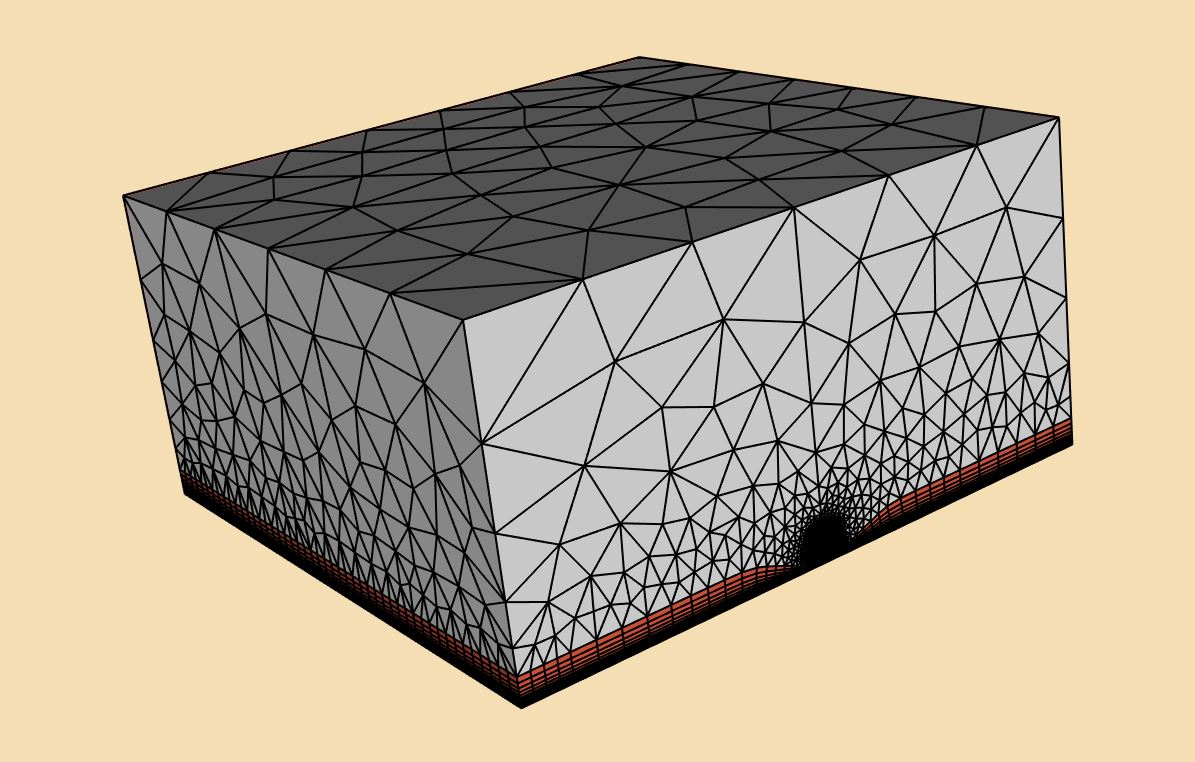
\includegraphics[width=\textwidth]{1a.jpg}
        \caption{Front}
        \label{fig:1c1}
    \end{subfigure}
    ~ 
    \begin{subfigure}[h]{0.2\textwidth}
        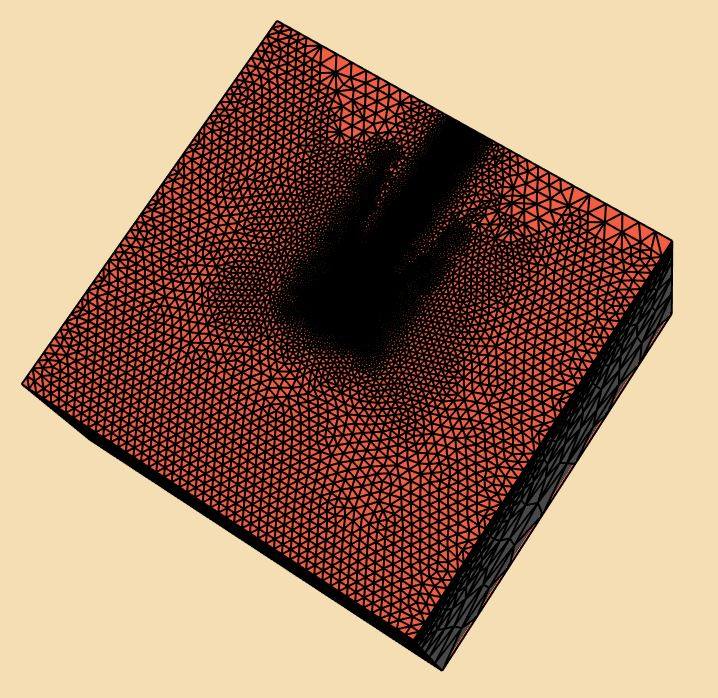
\includegraphics[width=\textwidth]{1b.jpg}
        \caption{Bottom}
        \label{fig:1c2}
    \end{subfigure}
    \caption{Direct import ICE-30deg-vel-pres.vtk}\label{fig:1c}
\end{figure}\\
\item Motivation\\\\
Train Accident in December 2005\\
“... The train was running at about 100 kilometers per hour when the accident occurred. There may have been strong vertical winds that may have lifted the train up as well as horizontal winds. ”\\
While the current fastest train in the world is traveling roughly 600 kilometers per hour, it would not take much side force to tilt the train and cause accident to happen. It drives the design of this visualization tool for train structure designers as a post-processor tool with the CFD data generated. It is going to provide concret presentation of flow around the train and pressure grandient around the train too. Which will help visualize the turbulent or vortex effect around the train body and to optimize the design specifically. There should be essential interaction tools for user to toggle their best interested area for in-depth observation.\\
\item Methodology\\\\
The basic methods would be focusing on the nature of the data type. Since the data is unstructured grid based, corresponding reader, and data pipe function would be used. Basic techniques such as isovalue clipping the results, transparent setup, color mapping trasnfer functions and tensor line function is expected. User interface setup such as clipping plane, line tube radius, scale of value result is also expected. It is believed that majority of time and effort would be researching the correct iso values and propagation values of transfer function to best visualize the dataset. Prepare pipelines\\
The proposed pipeline so far is illusitrated below:\\
For scalar pressure data, a contour filter is applied to extracted data from the geometry filter:
\begin{figure}[h]
    \centering
    \begin{subfigure}[h]{0.5\textwidth}
        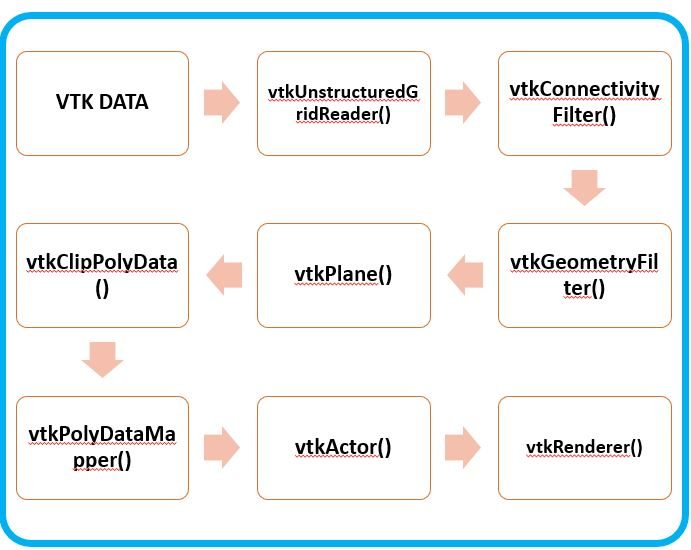
\includegraphics[width=\textwidth]{3a.jpg}
        \label{fig:1c1}
    \end{subfigure}
    ~ 
    \caption{Scalar Pressure Data Pipeline}\label{fig:1c}
\end{figure}\\
For vector velocity data, a probe filter is used to extracted data and attach to arrow:
\begin{figure}[h]
    \centering
    \begin{subfigure}[h]{0.5\textwidth}
        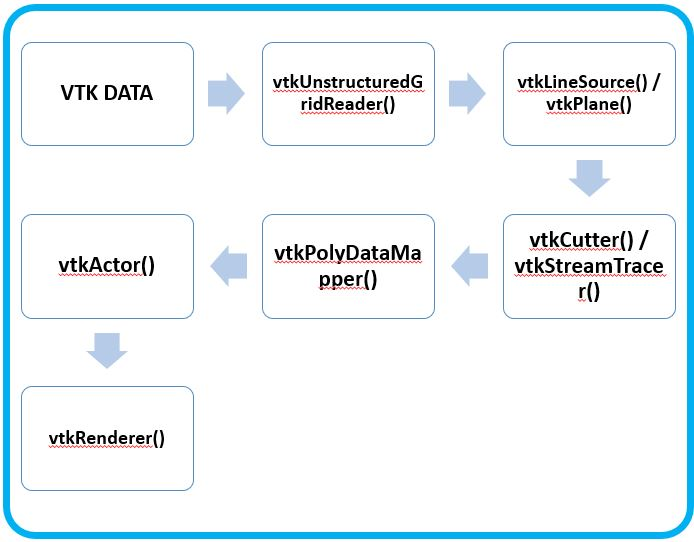
\includegraphics[width=\textwidth]{3b.jpg}
        \label{fig:1c1}
    \end{subfigure}
    ~ 
    \caption{Velocity Vector Data Pipeline}\label{fig:1c}
\end{figure}\\
The prelimenary timeline and major mile-stones are showed below:
\\
		\begin{tabular}{l l }
			\toprule
			\textit Week 3/30 & Week 4/6\\
			\midrule
				Identify data set & prepare initial setup pipelines \\
			\bottomrule\\
			\toprule
			\textit Week 4/13 & Week 4/20\\
			\midrule
			 generate initial visualizarion  & add-in user interface modules\\
			\bottomrule\\
			\toprule
			\textit Week 4/27\\
			\midrule
				polish report and submit\\
			\bottomrule
		\end{tabular}\\
\item Deliverable and Issue\\
As mentioned in Motivation section, the major deliverable is to provide visualization focusing on the train itself. The first issue was to filtering out the related data within the entire volume box. It was taking majority of time to research and understand the conditions happening inside the data. Below are measured dimension and boundary condition after iterating different planes and clips around the dataset:\\
\begin{figure}[h]
    \centering
    \begin{subfigure}[h]{0.4\textwidth}
        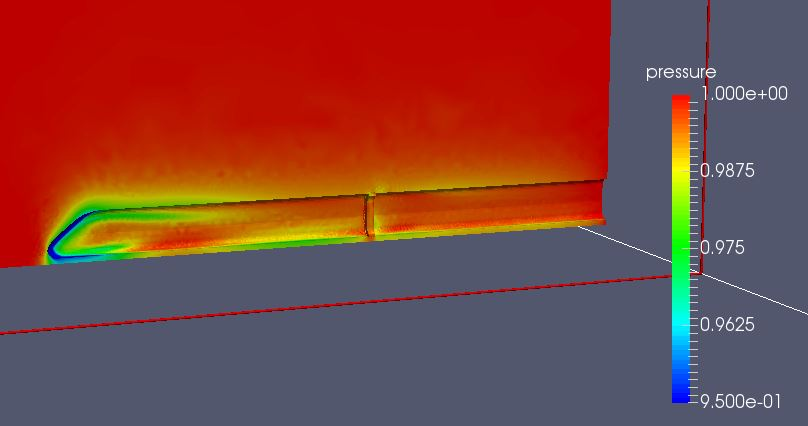
\includegraphics[width=\textwidth]{4e.jpg}
        \caption{ParaView Pressure}
        \label{fig:1c1}
    \end{subfigure}
    ~ 
    \begin{subfigure}[h]{0.4\textwidth}
        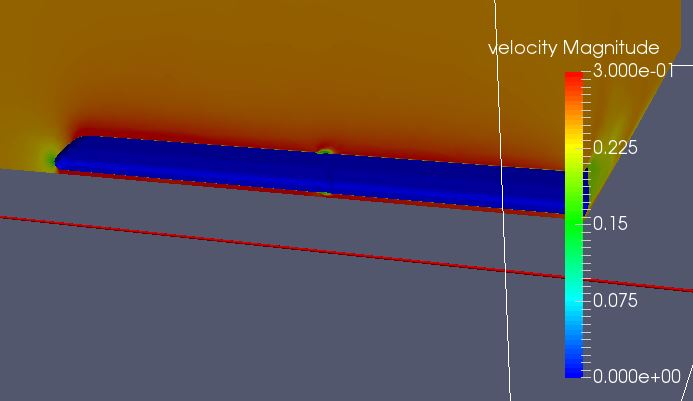
\includegraphics[width=\textwidth]{4f.jpg}
        \caption{ParaView Velocity}
        \label{fig:1c1}
    \end{subfigure}
    \caption{ParaView Measurement}\label{fig:1c}
     \begin{subfigure}[h]{0.5\textwidth}
        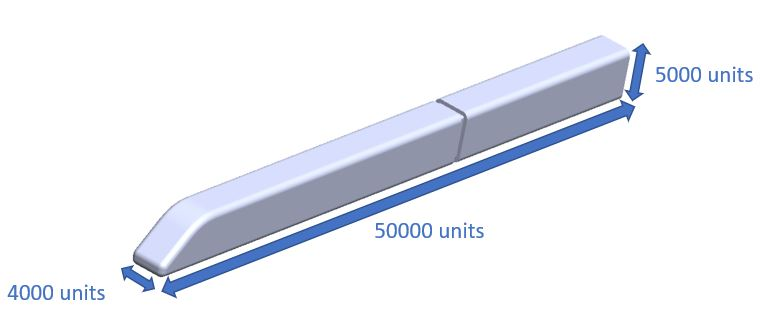
\includegraphics[width=\textwidth]{5a.jpg}
        \caption{Train Dimension}
        \label{fig:1c1}
    \end{subfigure}
    ~ 
    \begin{subfigure}[h]{0.4\textwidth}
        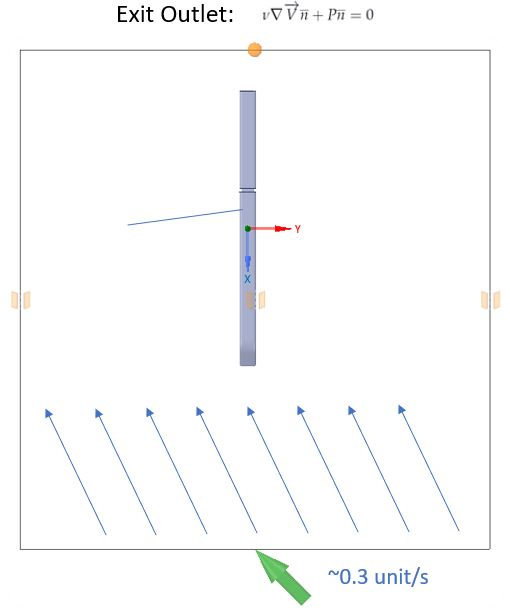
\includegraphics[width=\textwidth]{5b.jpg}
        \caption{Boundary Condition}
        \label{fig:1c1}
    \end{subfigure}
    \caption{Boundary Condition and Dimensions}\label{fig:1c}
\end{figure}\\\\\\\\\\\\\\\\\\\\\\\\\\\\
The other challenge is how to present different variable at the same time without interfering each other. If the data was plotted with opacity, there will be histering effect that layers of colors overlapping each other. And only representing the value with contour lines is not representative enough. Below are some trial presentation initially:
\begin{figure}[h]
    \centering
    \begin{subfigure}[h]{0.4\textwidth}
        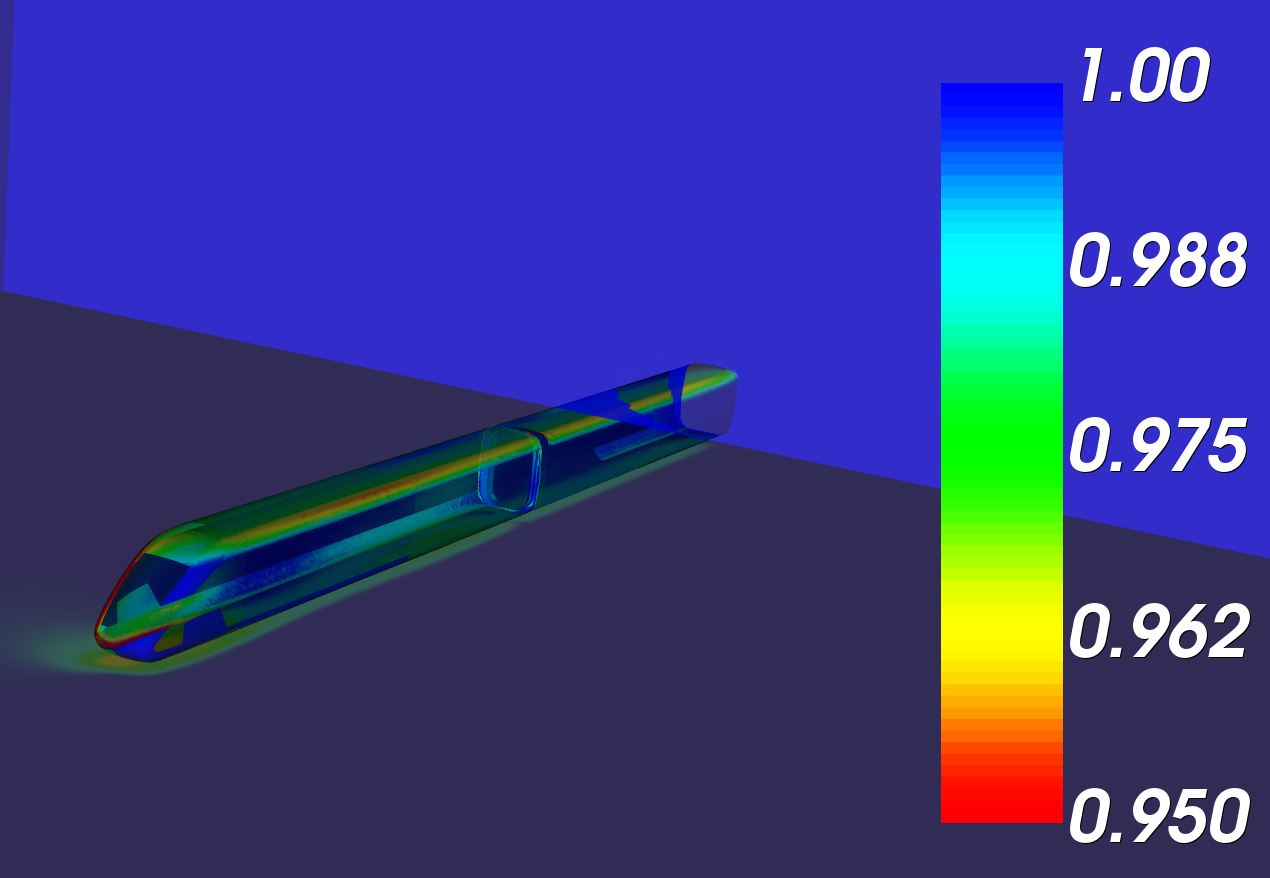
\includegraphics[width=\textwidth]{4a.jpg}
        \caption{Full geometry with opacity}
        \label{fig:1c1}
    \end{subfigure}
    ~ 
    \begin{subfigure}[h]{0.4\textwidth}
        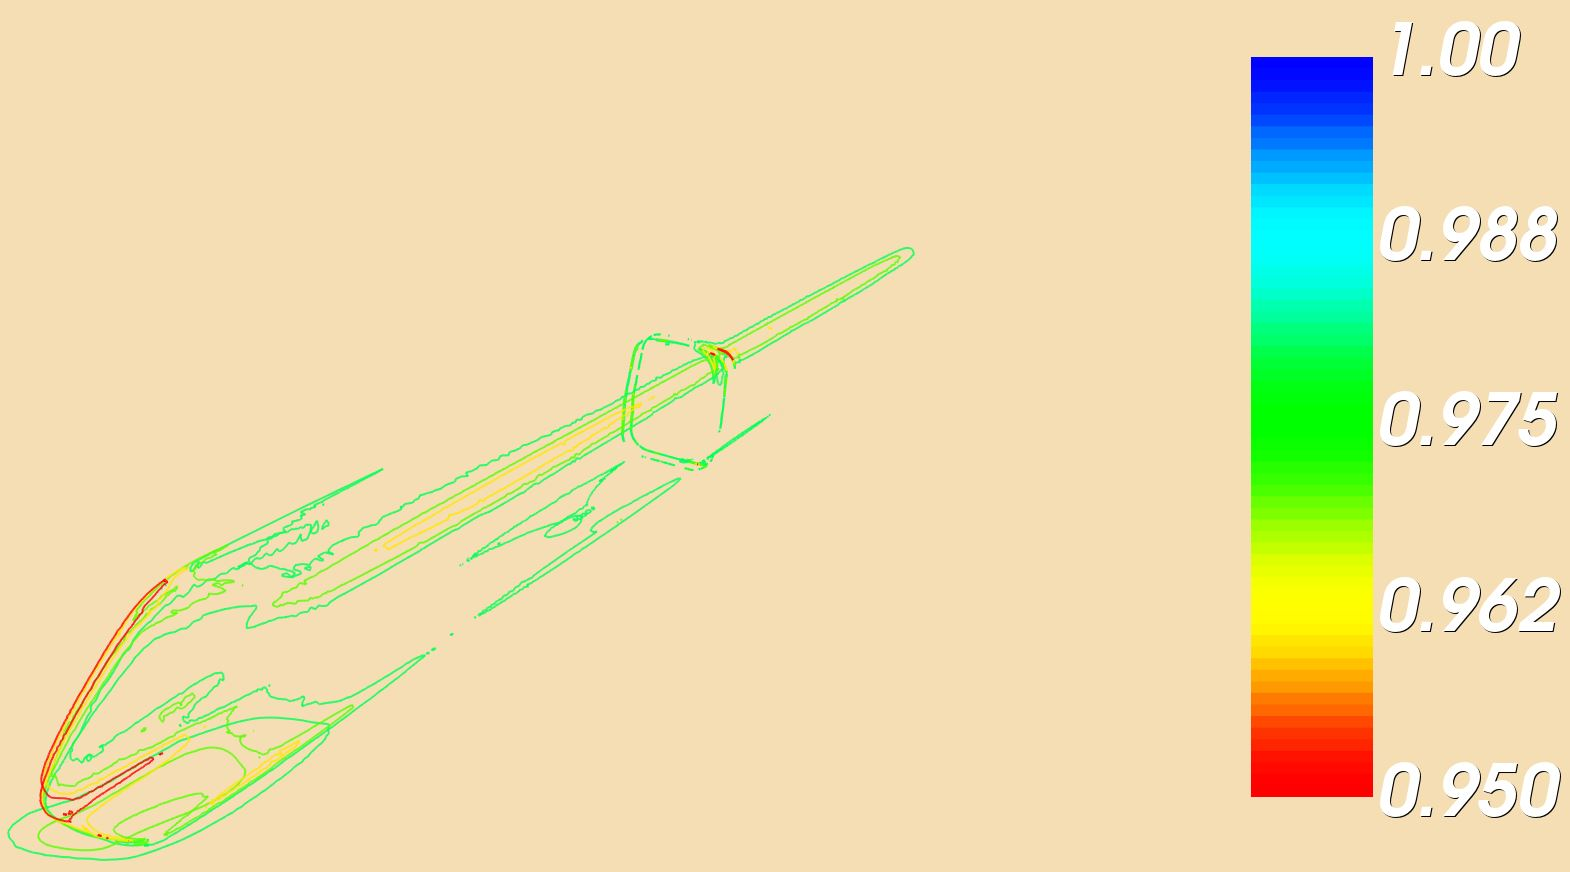
\includegraphics[width=\textwidth]{4b.jpg}
        \caption{Contour line only}
        \label{fig:1c1}
    \end{subfigure}
    \caption{ParaView Measurement}\label{fig:1c}
     \begin{subfigure}[h]{0.4\textwidth}
        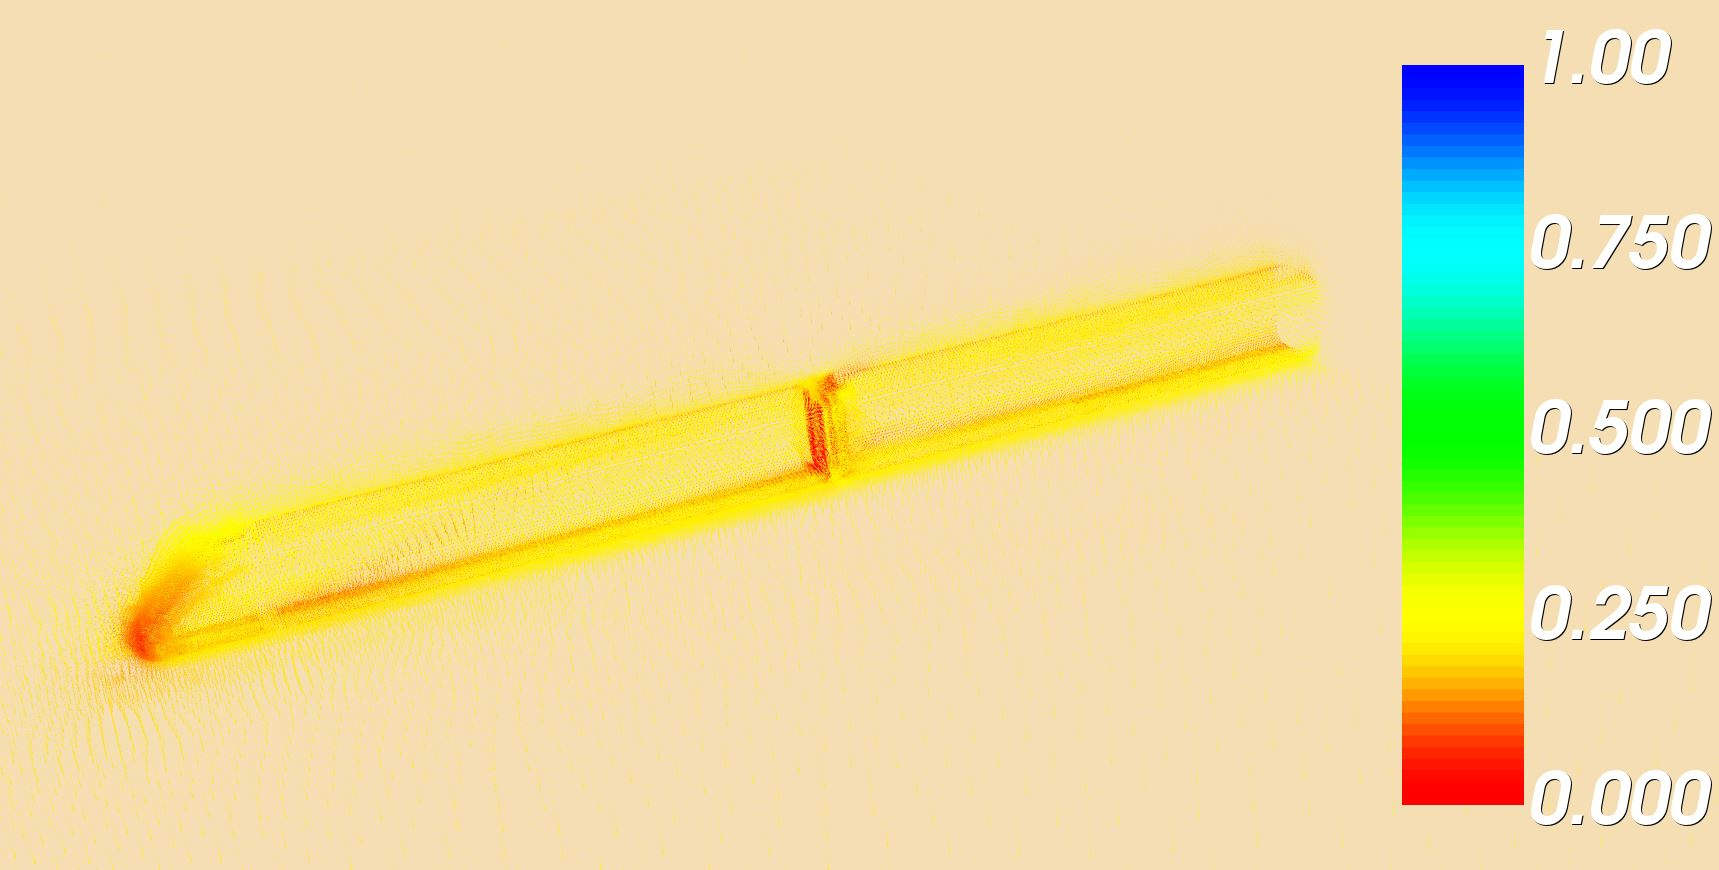
\includegraphics[width=\textwidth]{4c.jpg}
        \caption{Vector field}
        \label{fig:1c1}
    \end{subfigure}
    ~ 
    \begin{subfigure}[h]{0.4\textwidth}
        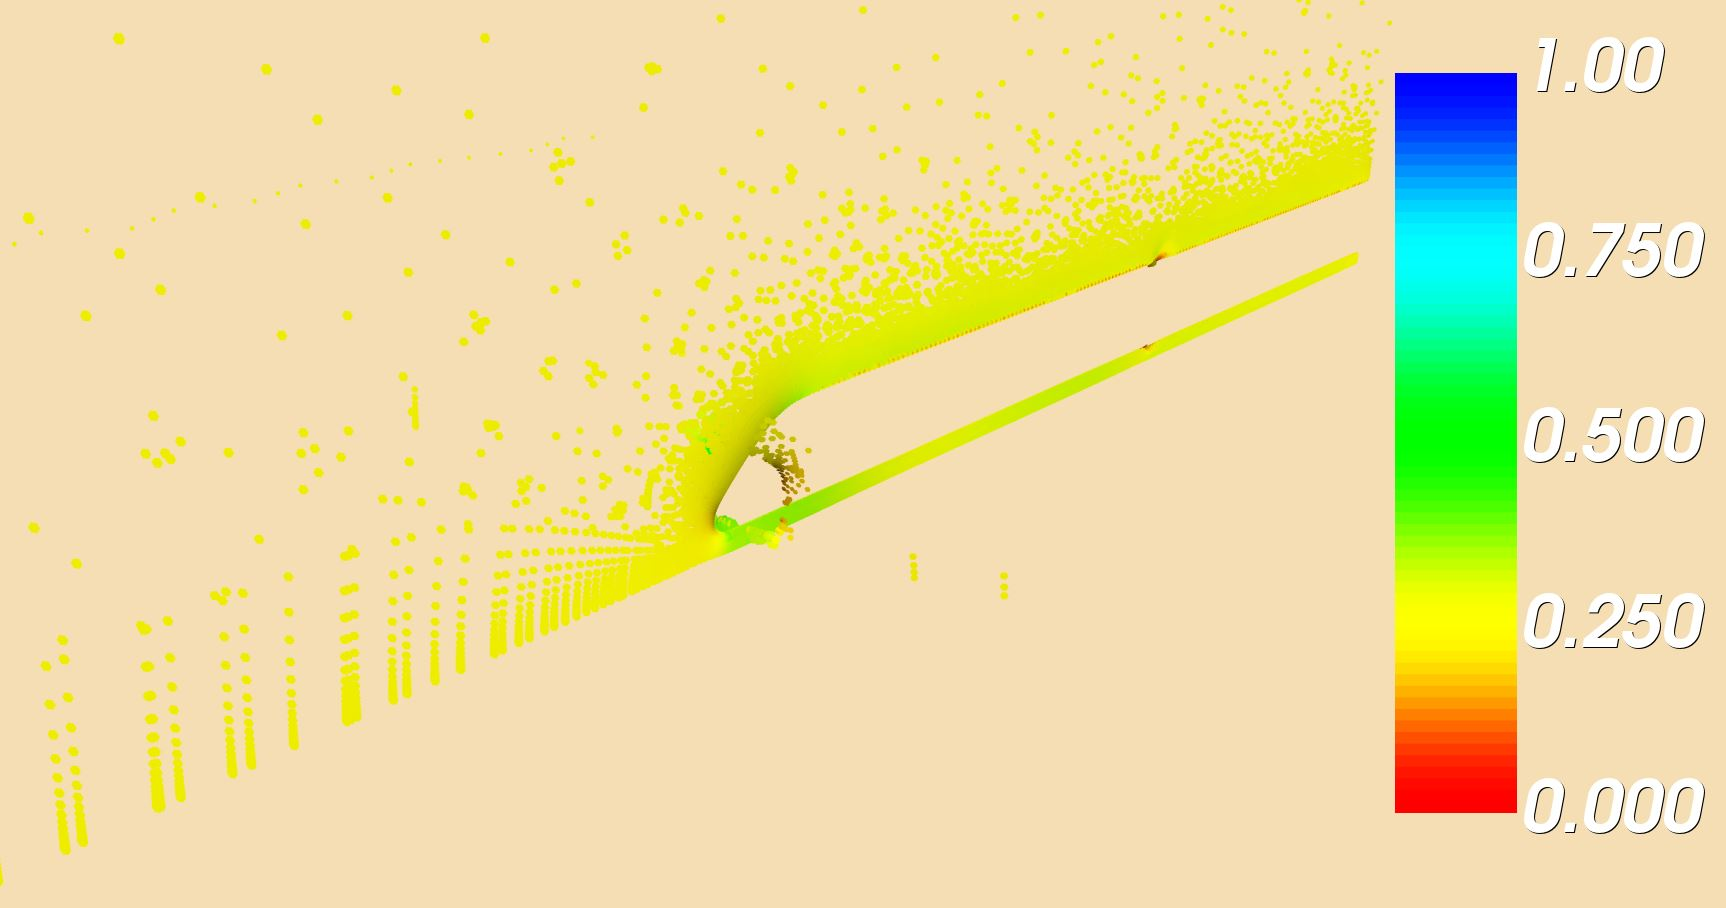
\includegraphics[width=\textwidth]{4d.jpg}
        \caption{Plane glyths}
        \label{fig:1c1}
    \end{subfigure}
    \caption{Different trial presentation}\label{fig:1c}
\end{figure}\\
\item Result\\
The final result is showed below, consisting the illustration and user interface tools are showed:\\
\begin{figure}[h]
    \centering
    \begin{subfigure}[h]{0.81\textwidth}
        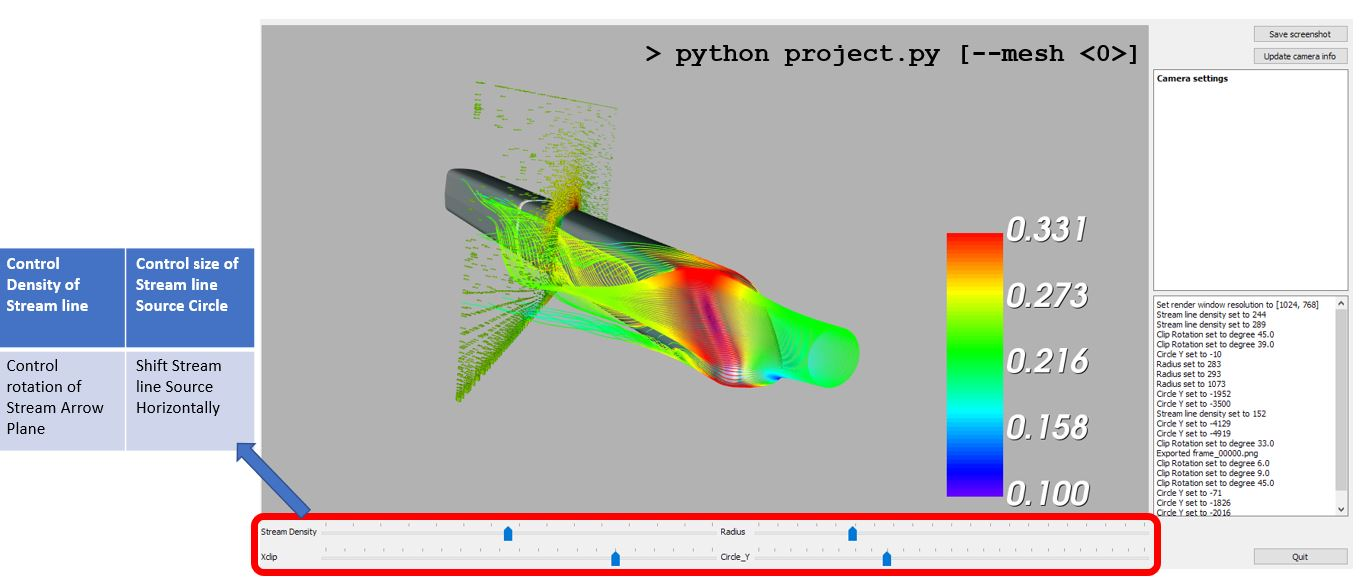
\includegraphics[width=\textwidth]{6a.jpg}
        \label{fig:1c1}
    \end{subfigure}
    \caption{Final Result}
\end{figure}\\
The way for streamlines sourced is based on a circular area parallel to the train head. It is showed to be the best capturing and wrapping method for streamline going across the train body. Alogn with the ultilities being able to change the size, density and position of this circular source allows the user to find the best angle and area for flow observation and conclusion. The glyth plane could also be rotate to suit the direction of incoming flow. The colorscheme for the train pressure distribution is different from the flow, which helps to isolate their exist but still being ablr to correlate simutaneously. There is one API input that could turn on and off the elements on the train body. Below are visualization results with different customized settings:\\
\begin{figure}[h]
    \centering
    \begin{subfigure}[h]{0.45\textwidth}
        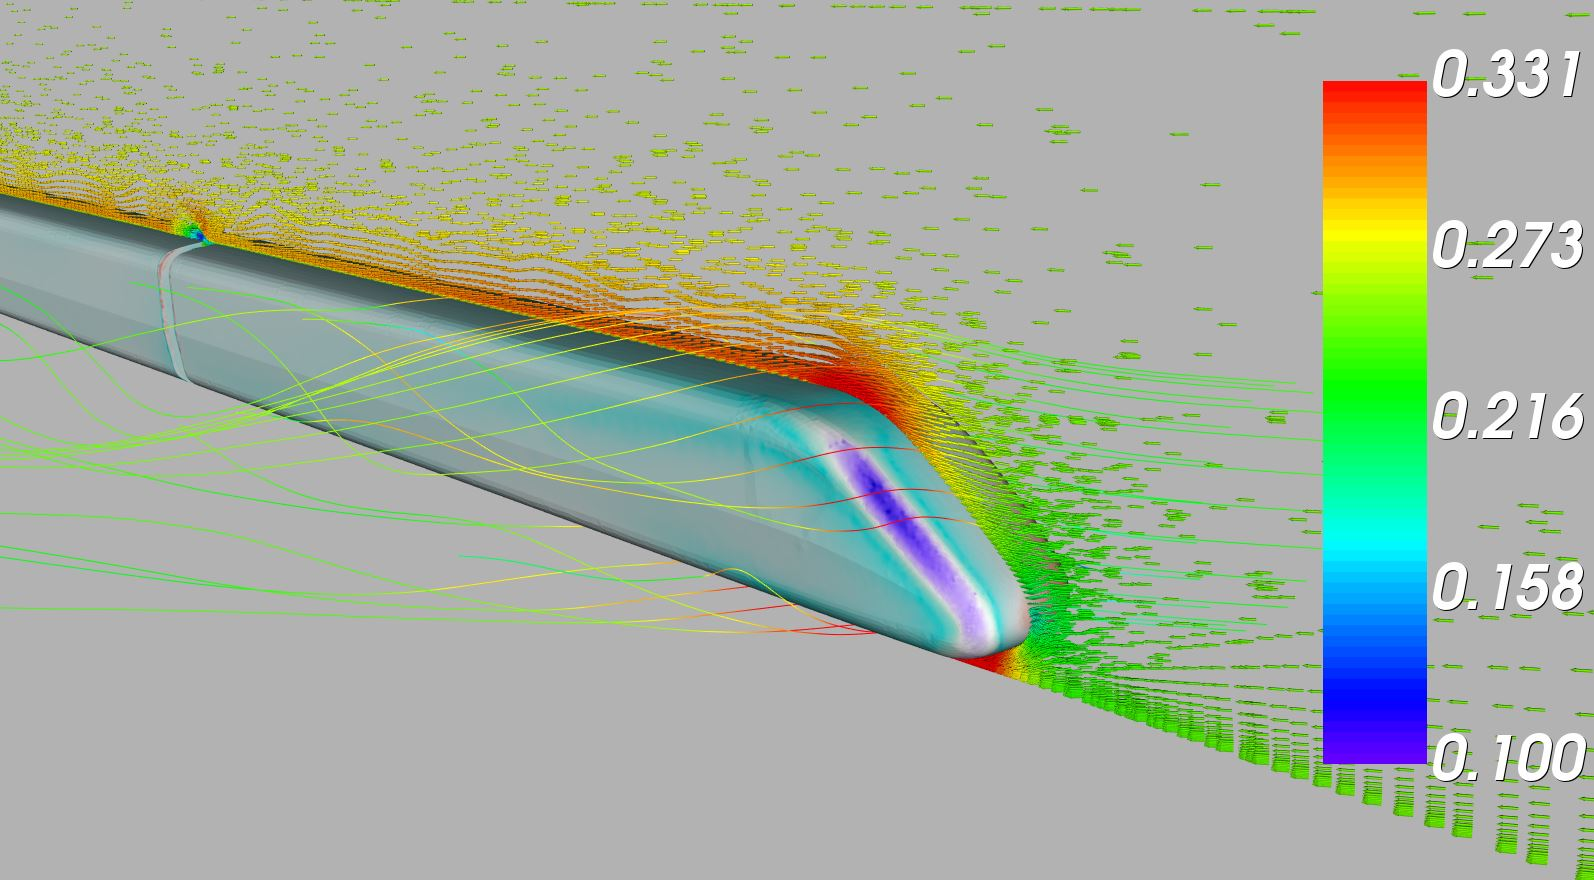
\includegraphics[width=\textwidth]{6b.jpg}
        \caption{Default Setting}
        \label{fig:1c1}
    \end{subfigure}
    ~ 
    \begin{subfigure}[h]{0.45\textwidth}
        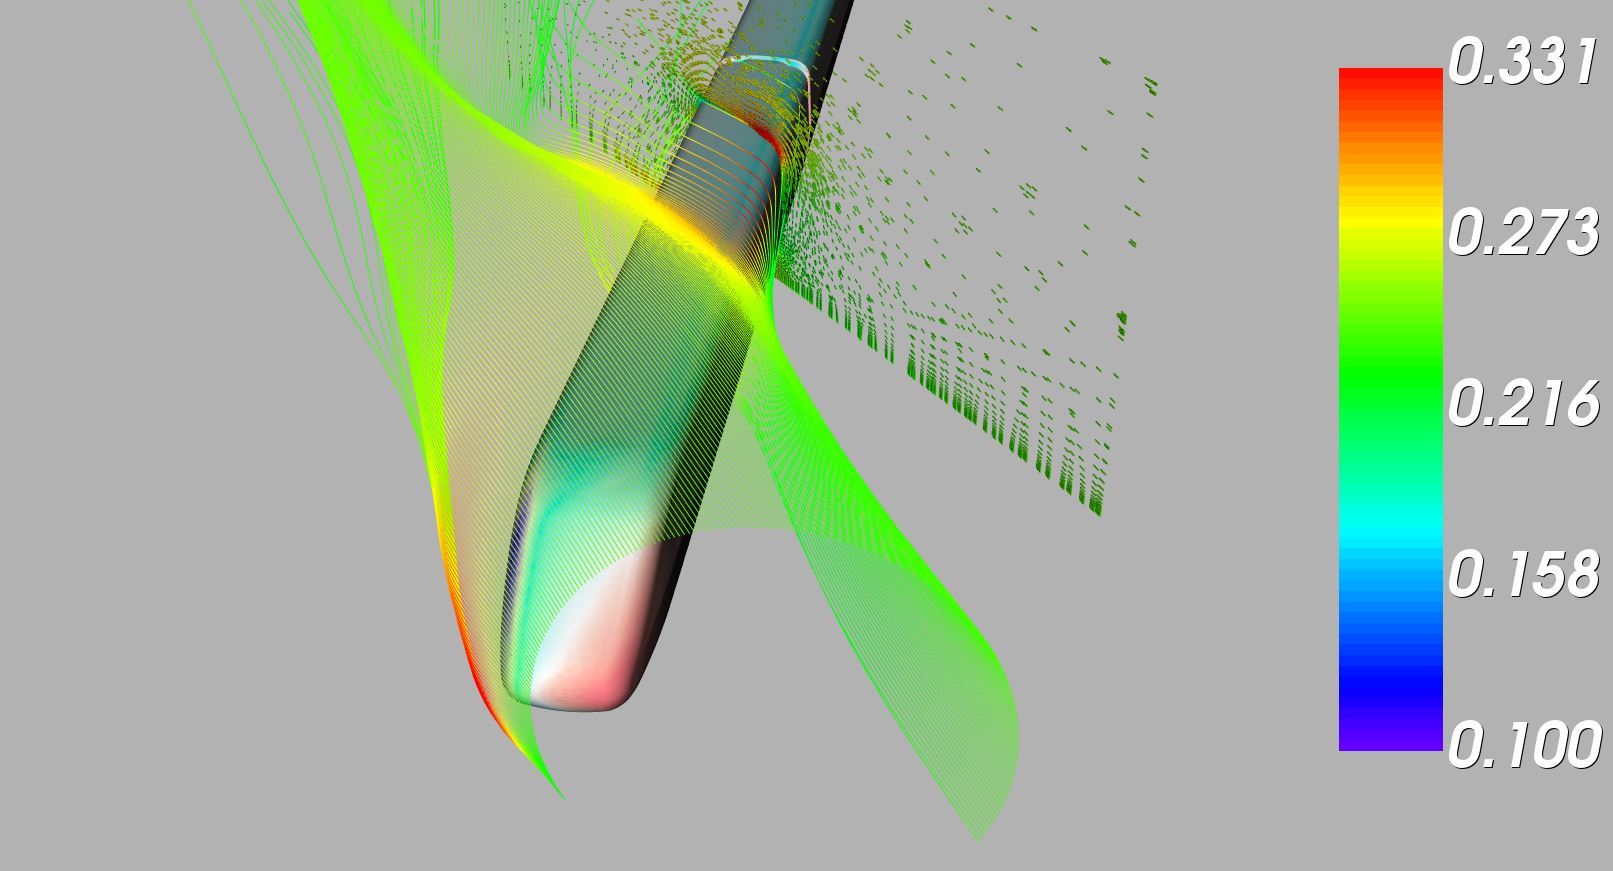
\includegraphics[width=\textwidth]{6c.jpg}
        \caption{Large Source}
        \label{fig:1c1}
    \end{subfigure}
    \caption{ParaView Measurement}\label{fig:1c}
     \begin{subfigure}[h]{0.45\textwidth}
        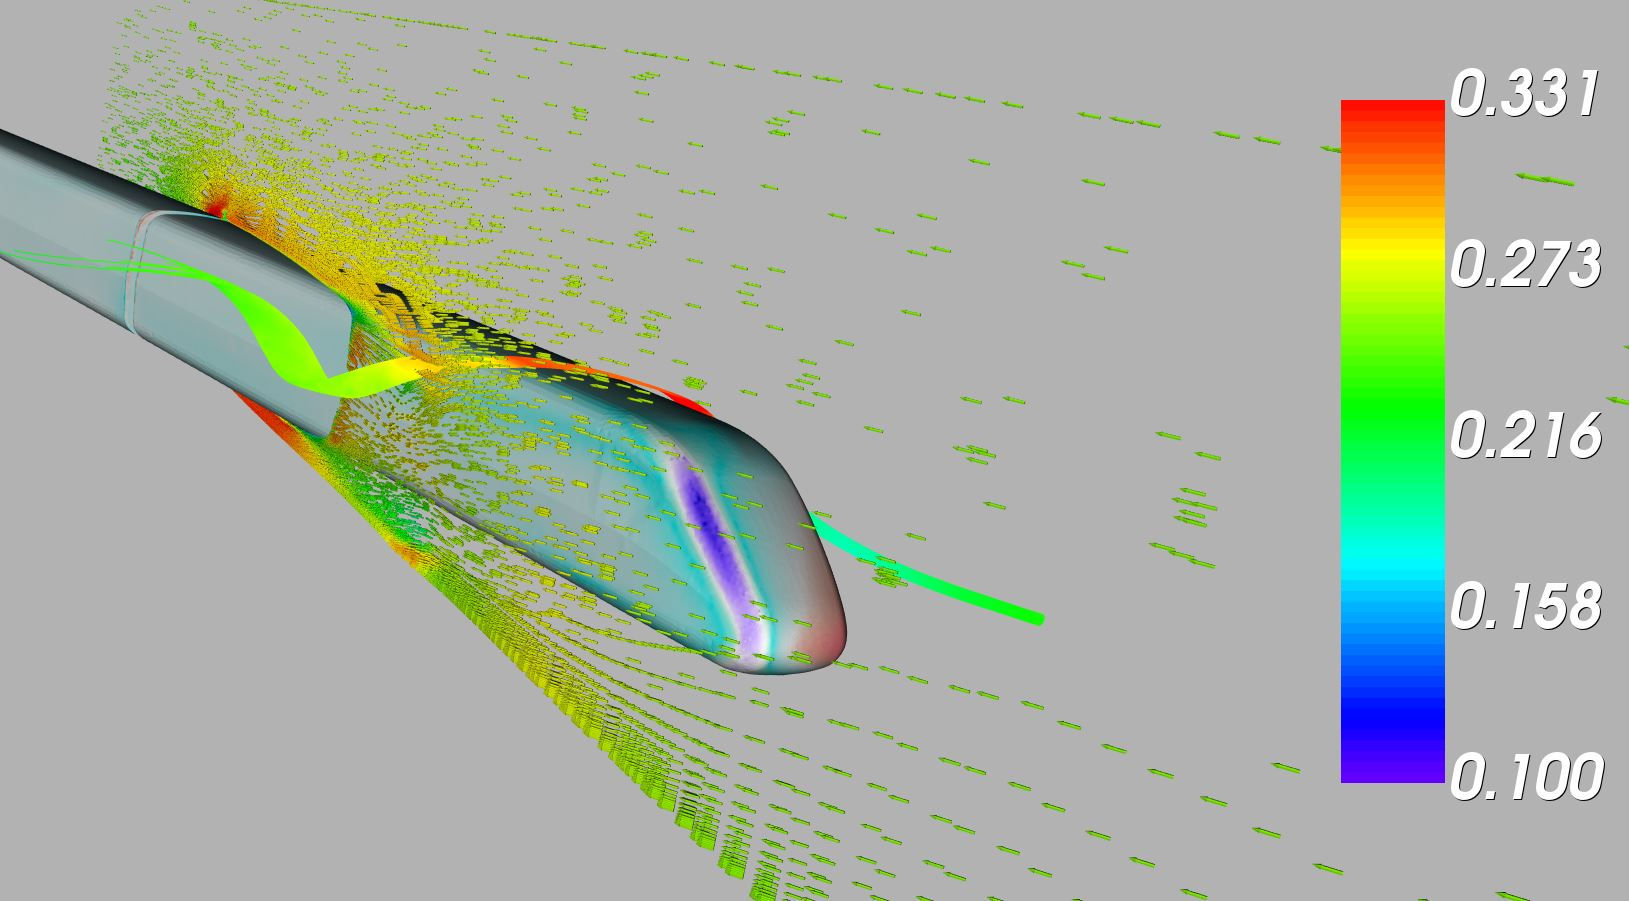
\includegraphics[width=\textwidth]{6d.jpg}
        \caption{Small Source}
        \label{fig:1c1}
    \end{subfigure}
    ~ 
    \begin{subfigure}[h]{0.45\textwidth}
        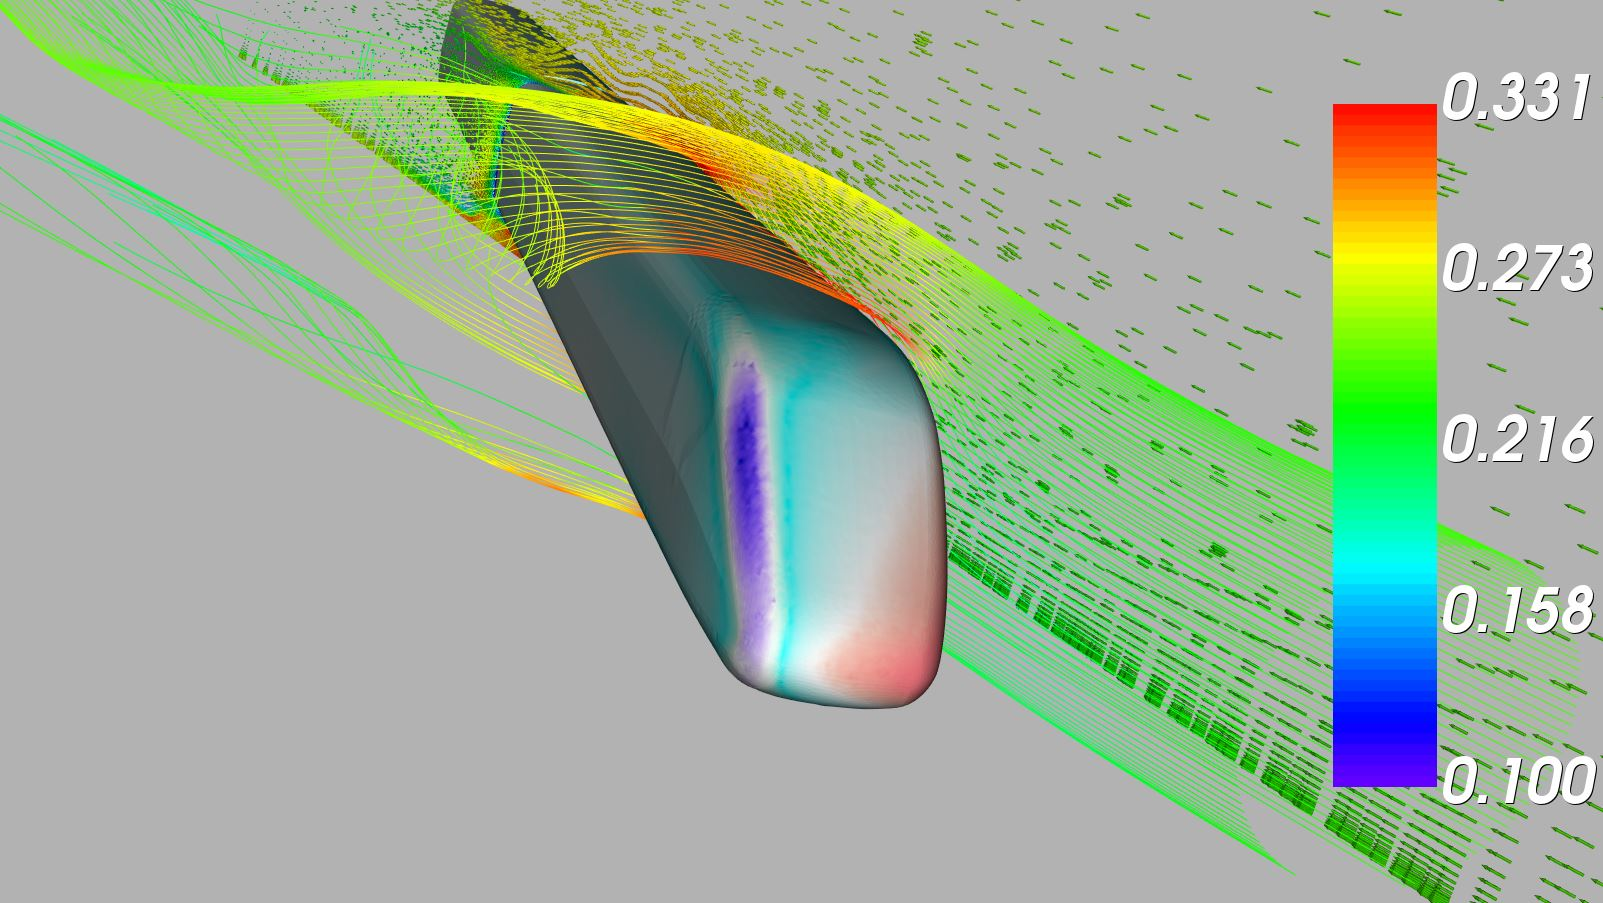
\includegraphics[width=\textwidth]{6e.jpg}
        \caption{Shifted Source}
        \label{fig:1c1}
    \end{subfigure}
    \caption{Different trial presentation}\label{fig:1c}
\end{figure}\\
\item Conclusion\\
Overall this assignment achieved the major deliveralbe targets. The tool is able to present the CFD data as expected. It ultilize VTK application in different aspect, which was learnt in this semester. The interesting follow-up action would be designing a tool that is transient data capable. While the current tool is designed against the static dataset, at one time-step only. The integration of time dependent visualization would be even more beneficial. Finally I would like to give great appreciation to all the faculty and TAs in class, who are always being helpful and passionate in visualization. 
\end{enumerate}
%----------------------------------------------------------------------------------------


%----------------------------------------------------------------------------------------


	
%----------------------------------------------------------------------------------------

\end{document}
